% kompilace xelatex prezentace.tex
% dokumentace k beameru: http://ftp.cvut.cz/tex-archive/macros/latex/contrib/beamer/doc/beameruserguide.pdf

% nastavení formátu prezentace 16:9
\documentclass[czech,aspectratio=169]{beamer}

\usepackage{polyglossia}
\setmainlanguage{czech}

% nastavení vzhledu
% další možnosti vzhledu viz https://hartwork.org/beamer-theme-matrix/
\usetheme{Madrid}
\usecolortheme{whale}
\usepackage{subfig}

\usepackage{caption}

% for setting different borders
\usepackage{geometry}

% left, right v includegraphics
\usepackage[export]{adjustbox}

\usepackage{csquotes}

\usepackage{media9} % prehravani videa

% vzhled slajdů vnitřní téma (např. vzhled odrážek)
\useinnertheme{rectangles} %možnosti: default circles rectangles rounded inmargin
% vzhled slajdů vnější téma
\useoutertheme{default} %možnosti: default, miniframes, smoothbars, sidebar, split, shadow, tree, smoothtree, infolines

% zavedeme čvutí modou barvu
\definecolor{CVUT}{HTML}{0065BD}
% čvutí modou použijeme jako hlavní barvu prezentace
\setbeamercolor{structure}{bg=white,fg=CVUT}

% jako font prezentace nadefinujeme oficiální ČVUT písmo Technika -- pokud chcete použít, musíte si font nainstalovat nebo jej nahrát na Overleaf
% https://www.cvut.cz/logo-a-graficky-manual  -- inforek, přihlášení přes celoškolské heslo
%\usepackage{fontspec}
%\setsansfont{Technika-Kniha}

% vypneme navigační panel beamer (pro zapnutí zakomentujeme)
\beamertemplatenavigationsymbolsempty

% vygenerujeme slajdy s poznámkami -- ty si můžete vytisknout a mít je na obhajobu s sebou (pokud zapomenete slova, nebo kdyby nefungovalo promítání z nějakého důvodu)
%\setbeameroption{show notes}

% vygeneruje slajdy s poznámky vhodné pro promítání na dvou monitorech -- na obhajobu nevyužijete
%\usepackage{pgfpages}
%\setbeameroption{show notes on second screen}

% variable block width
\newenvironment<>{varblock}[2][.9\textwidth]{%
	\setlength{\textwidth}{#1}
	\begin{actionenv}#3%
		\def\insertblocktitle{#2}%
		\par%
		\usebeamertemplate{block begin}}
	{\par%
		\usebeamertemplate{block end}%
\end{actionenv}}

% fromat datumu
\usepackage[style=dmyyyy,datesep={.}]{datetime2}

% další balíčky
\usepackage{graphicx}
\usepackage{hyperref}
\usepackage{tikz}
\usetikzlibrary{chains,fit,shapes}

% Údaje o prezentaci
\title[GAN Dissection]{GAN Dissection: Visualizing and Understanding Generative Adversarial Networks}
\institute[FIT CTU]{Faculty of Information Technology \\ Czech Technical University in Prague}
\author[M. Šafránek]{Martin Šafránek}
%\date{\today}
\date{}
\titlegraphic{
\includegraphics[width=.1\textwidth]{../media/logo-cvut}}


\begin{document}

\begin{frame}
	\titlepage
	\note{Nezapomenout pozdravit} %tohle je poznámka, ta na slajdu nebude, ale vygeneruje se vedle něj, pokud odkomentujete příkaz výše -- \setbeameroption{show notes}
\end{frame}


%%%%%%%%%%%%%%%%%%%%%%%%%%%%%%%%%%%%%%%%%%%%%%%%%%%%%%%%%%%%%%%%%%%%%%%%%%%%%%
\section{Introduction}
%%%%%%%%%%%%%%%%%%%%%%%%%%%%%%%%%%%%%%%%%%%%%%%%%%%%%%%%%%%%%%%%%%%%%%%%%%%%%%

\begin{frame}{Parts}
	\begin{itemize}
		\item GAN overview
		\item GAN dissection (paper)
	\end{itemize}

\end{frame}

%%%%%%%%%%%%%%%%%%%%%%%%%%%%%%%%%%%%%%%%%%%%%%%%%%%%%%%%%%%%%%%%%%%%%%%%%%%%%%
\section{GAN introduction}
%%%%%%%%%%%%%%%%%%%%%%%%%%%%%%%%%%%%%%%%%%%%%%%%%%%%%%%%%%%%%%%%%%%%%%%%%%%%%%

\begin{frame}{Adversarial Nets Framework}
	\centering
	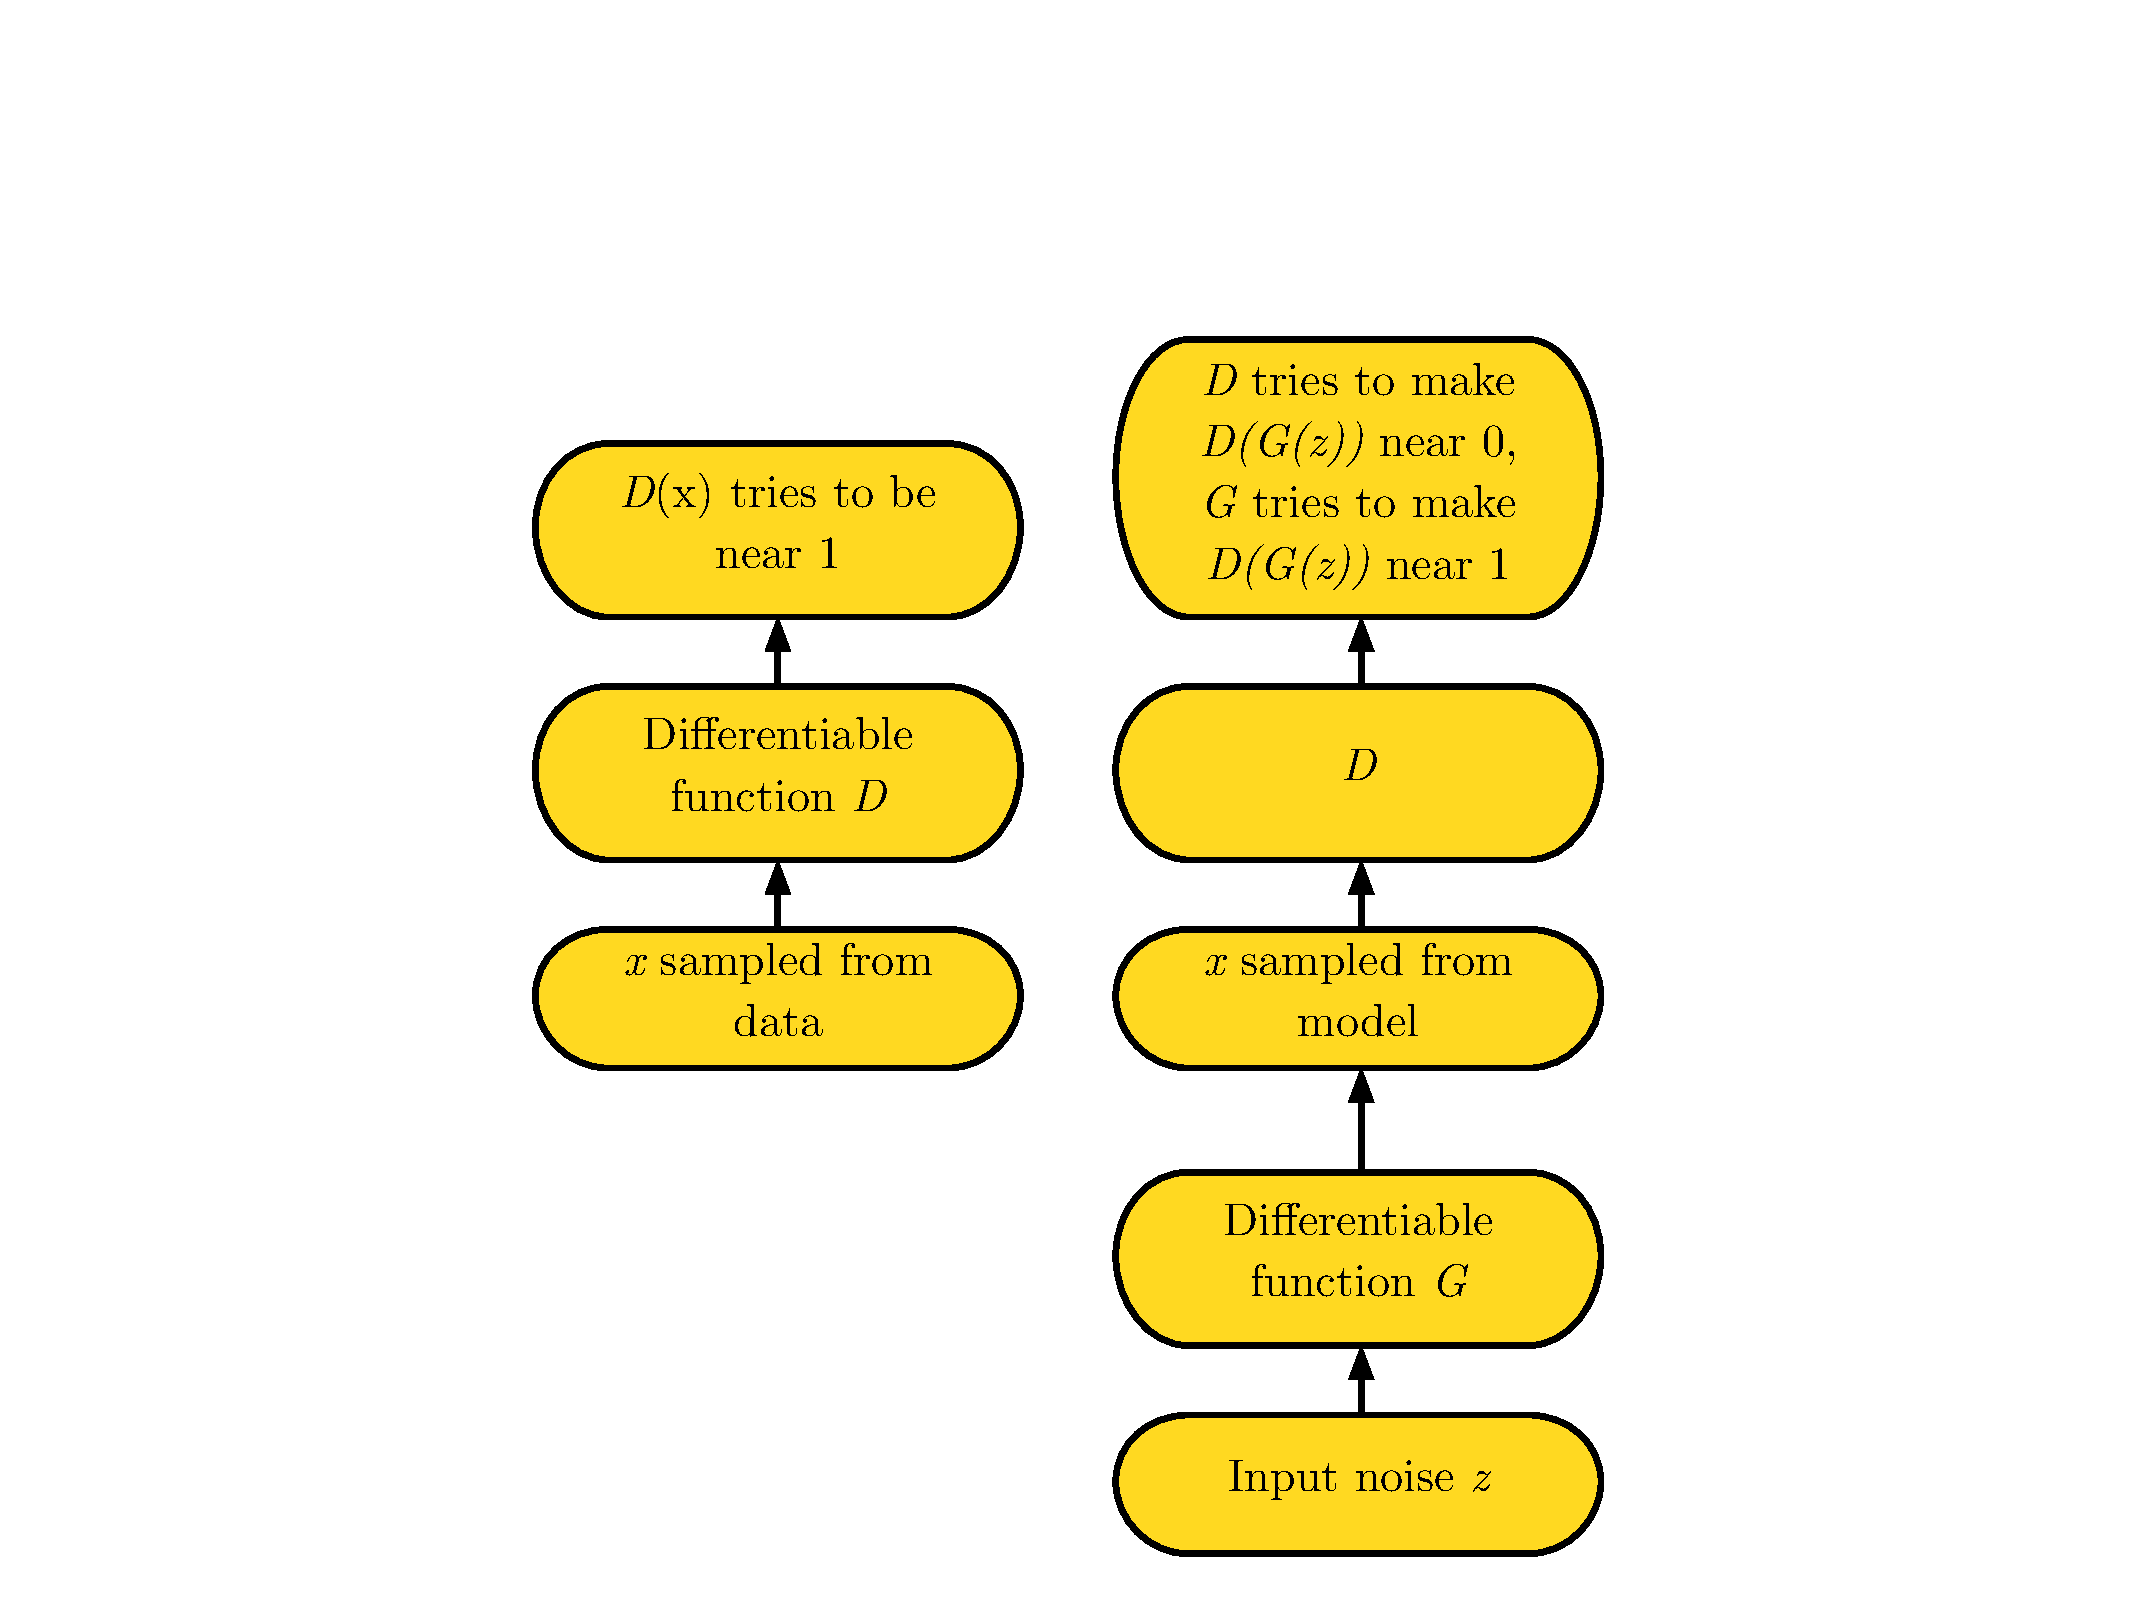
\includegraphics[width=0.8\textheight]{../media/gan_architecture.pdf}
\end{frame}

\begin{frame}{Minimax Game}
	\begin{figure}
		$$
		J^{\left( D \right)} = - \dfrac{1}{2}\mathbb{E}_{x\~{}p_{\rm data}} \, \mathrm{log} \, D(x) - \dfrac{1}{2}\mathbb{E}_z \, \mathrm{log} \, (1-D(G(z)))
		$$
		$$
		J^{G} = -J^{D}
		$$
	\end{figure}
	\begin{itemize}
		\item Generator minimizes the log-probability of the discriminator
		being correct
		\item Equilibrium if the discriminator is unable to differentiate between real and generated input
	\end{itemize}
\end{frame}


%%%%%%%%%%%%%%%%%%%%%%%%%%%%%%%%%%%%%%%%%%%%%%%%%%%%%%%%%%%%%%%%%%%%%%%%%%%%%%
\section{GAN dissection paper}
%%%%%%%%%%%%%%%%%%%%%%%%%%%%%%%%%%%%%%%%%%%%%%%%%%%%%%%%%%%%%%%%%%%%%%%%%%%%%%

\begin{frame}{The paper}
	\begin{itemize}
		\item presents method for visualizing and understanding GAN
		\item assumes GAN generator is implemented as Convolutional neural network
		\item presents that learned GAN contains variables for doors, trees, ...
		\item shows how we can interactively manipulate objects in a scene
	\end{itemize}
\end{frame}


\begin{frame}
	\centering
	\begin{figure}
		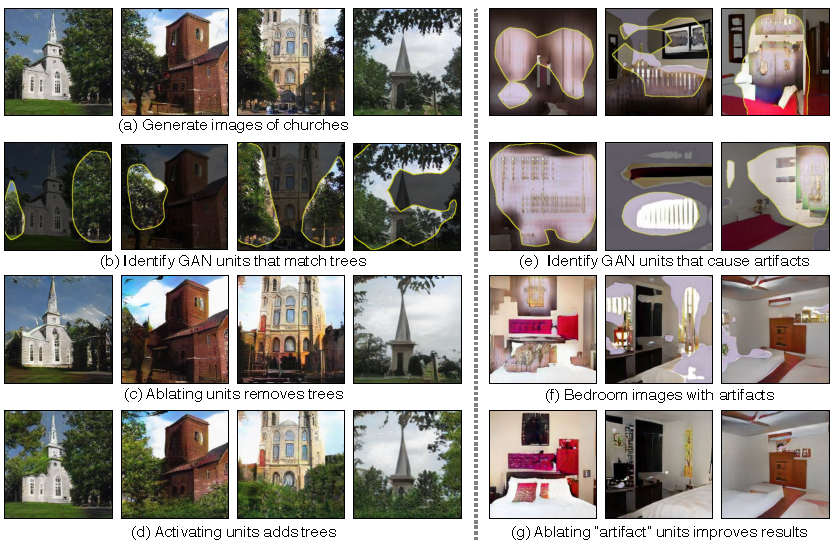
\includegraphics[width=1.3\textheight]{../media/figure_overview}
	\end{figure}
\end{frame}

%%%%%%%%%%%%%%%%%%%%%%%%%%%%%%%%%%%%%%%%%%%%%%%%%%%%%%%%%%%%%%%%%%%%%%%%%%%%%%
\section{Method}
%%%%%%%%%%%%%%%%%%%%%%%%%%%%%%%%%%%%%%%%%%%%%%%%%%%%%%%%%%%%%%%%%%%%%%%%%%%%%%


\begin{frame}{Terminology}
	\begin{itemize}
		\item function $\textbf{G}: z \rightarrow x$ (generator $G$ generates image $x$ from latent vector $z$)
		\item tensor $\textbf{r}$, where $r=h(z), x=f(r)=f(h(z)) = G(z)$ (featuremaps)
		\item $r$ has all the data neccessary to produce image $x$
		\item concept $\textbf{c} \in \mathbb{C}$ (chair, door, ...)
		\item $\textbf{r}_{\mathbb{U}, P} = ( r_{U,P}, r_{\overline{U}, P}  )$
		\item \textbf{$U$} selected featuremaps (units)

	\end{itemize}
\begin{figure}[b!]
	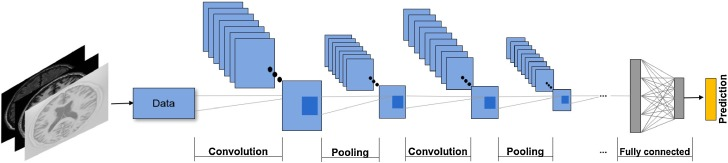
\includegraphics[height=0.26\textheight]{../media/covnet}
	\captionsetup{labelformat=empty}
	\caption{Covnet example \href{https://ars.els-cdn.com/content/image/1-s2.0-S0933365716305206-gr2.jpg}{\scriptsize {[Source]}}}
\end{figure}
\end{frame}

\begin{frame}{Architecture}
	\centering
	\begin{figure}
		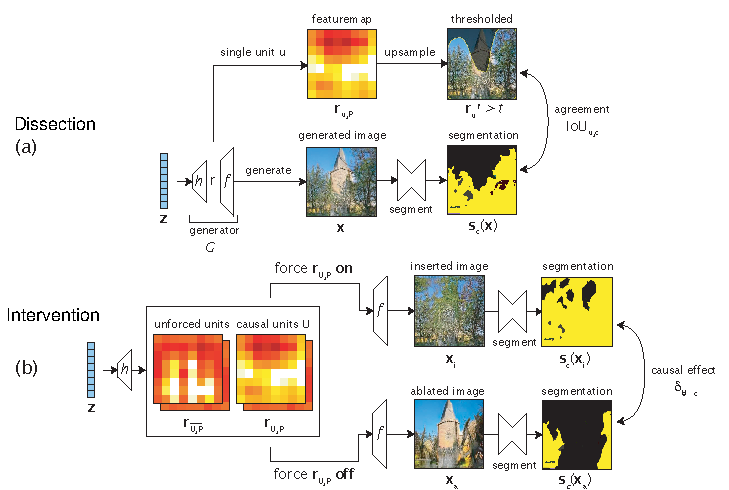
\includegraphics[width=1.2\textheight]{../media/paper_architecture}
	\end{figure}
\end{frame}

\begin{frame}{Dissection}
		
\end{frame}

\begin{frame}{Intervention}
	
\end{frame}

%%%%%%%%%%%%%%%%%%%%%%%%%%%%%%%%%%%%%%%%%%%%%%%%%%%%%%%%%%%%%%%%%%%%%%%%%%%%%%
\section{Results}
%%%%%%%%%%%%%%%%%%%%%%%%%%%%%%%%%%%%%%%%%%%%%%%%%%%%%%%%%%%%%%%%%%%%%%%%%%%%%%

\begin{frame}{Interpretable units for different scene categories}
	\centering
	\begin{figure}
		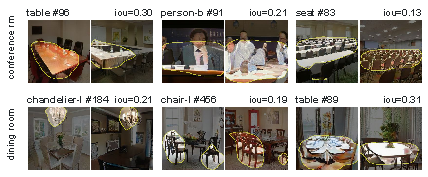
\includegraphics[width=\textwidth]{../media/figure5-left}
	\end{figure}
\end{frame}

\begin{frame}{Interpretable units for different network layers}
	\centering
	\begin{figure}
		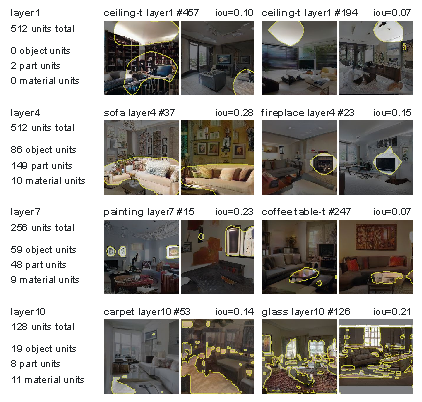
\includegraphics[height=0.85\textheight]{../media/figure6}
	\end{figure}
\end{frame}


\begin{frame}{Diagnosing and improving GANs}
		\begin{itemize}
			\item identify artifacts with human annotation
			\item 10 minutes to locate 20 artifact-causing units
			\item ablate found artifacts
		\end{itemize}
	\centering
	\begin{figure}
		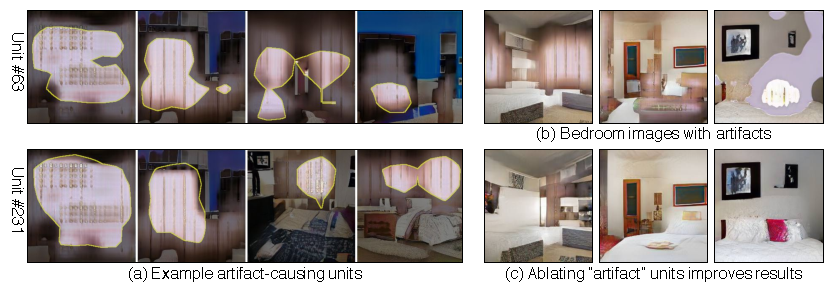
\includegraphics[height=0.6\textheight]{../media/figure8}
	\end{figure}
\end{frame}


\begin{frame}{Locating casual units with ablation}
		\begin{itemize}
			\item force erasing/size reduction
			\item Does GAN learns patterns ? eg \enquote{\textit{All bedrooms must have windows.}}
		\end{itemize}
		\begin{figure}
			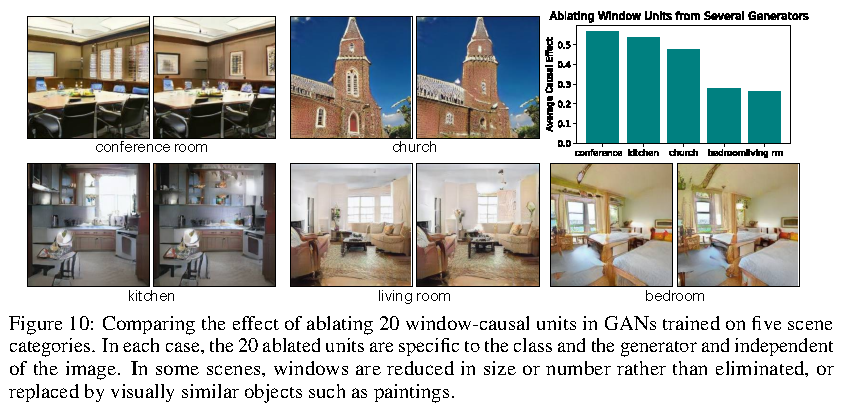
\includegraphics[height=0.7\textheight]{../media/figure10}
		\end{figure}
\end{frame}

\begin{frame}{Characterizing contextual relationships via insertion}
	\begin{itemize}
		\item force insertion of features into specific locations in scenes
		\item GAN forces realtionships eg \enquote{\textit{Doors can't be added to sky.}}, because the choice is vetoed later
	\end{itemize}
	\begin{figure}
		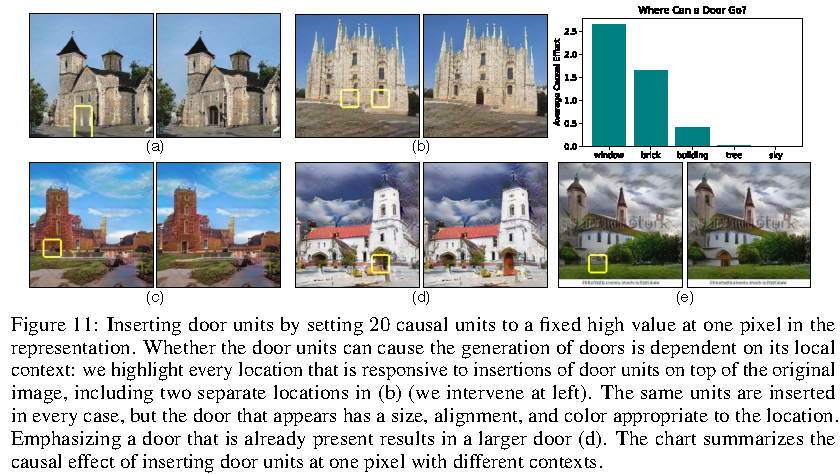
\includegraphics[height=0.7\textheight]{../media/figure11}
	\end{figure}
\end{frame}

\begin{frame}{Interactive toolkit}
	\centering
	\begin{figure}
		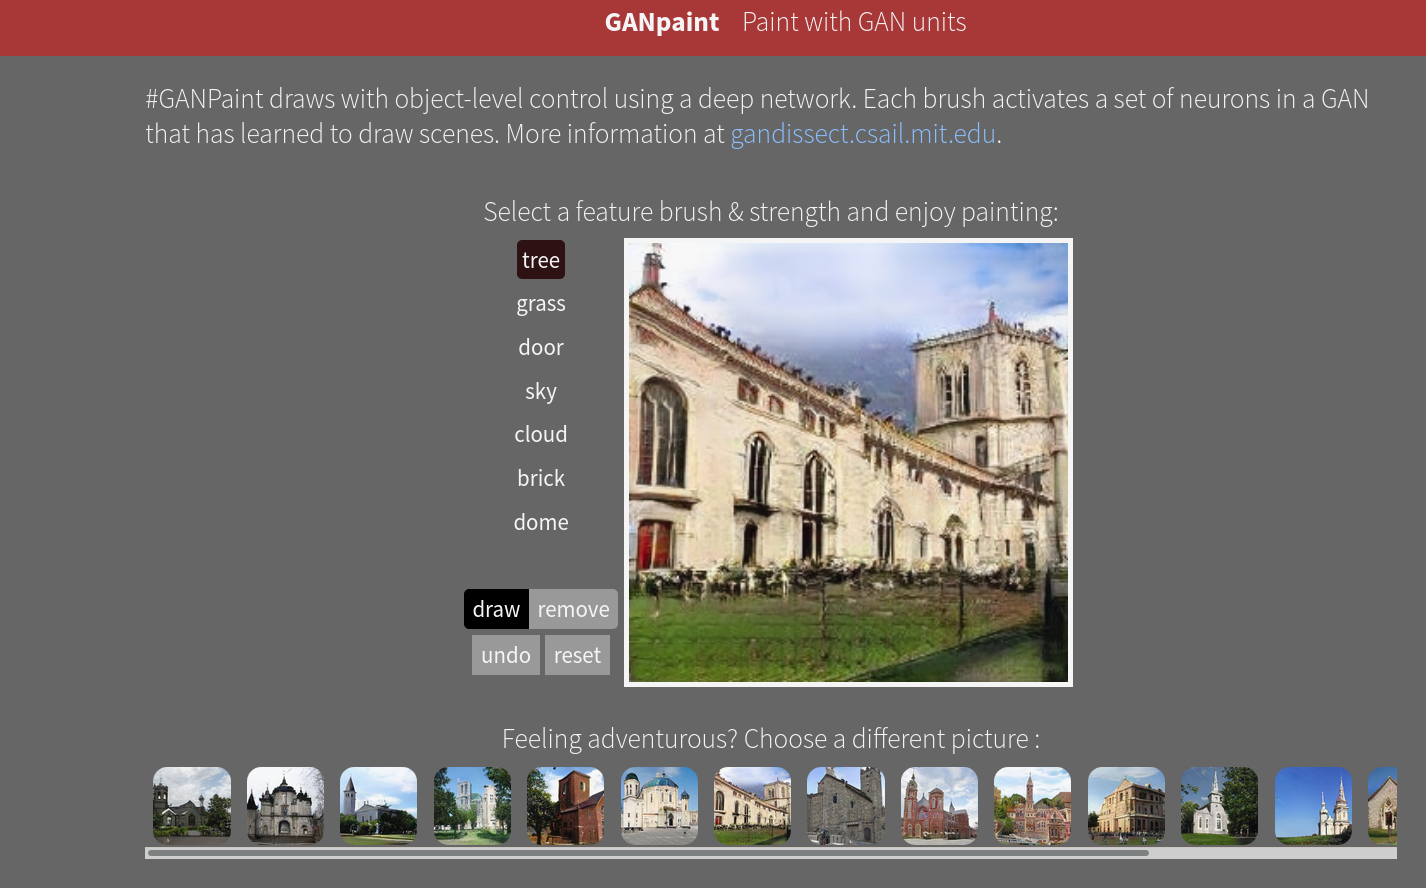
\includegraphics[width=1.2\textheight]{../media/ganter_screenshot.png}
		\small \url{http://gandissect.res.ibm.com/ganpaint.html}
	\end{figure}
\end{frame}

\begin{frame}{Further reasearch suggested by authors}
	\begin{enumerate}
		\item \enquote{\textit{Why can a door not be inserted in the sky ?}}
		\item \enquote{\textit{How does GAN suppress the signal in the later layers ?}}
		\item \enquote{\textit{What are the relationships between layers of a GAN ?}}
	\end{enumerate}
\end{frame}

\begin{frame}
	\centering
	{\Huge Questions ?}
\end{frame}

\end{document}
